% Modeled after the following
% A simple Tree
% Author: Stefan Kottwitz
% https://www.packtpub.com/hardware-and-creative/latex-cookbook
\documentclass[border=10pt]{standalone}
\usepackage{tikz}
\begin{document}
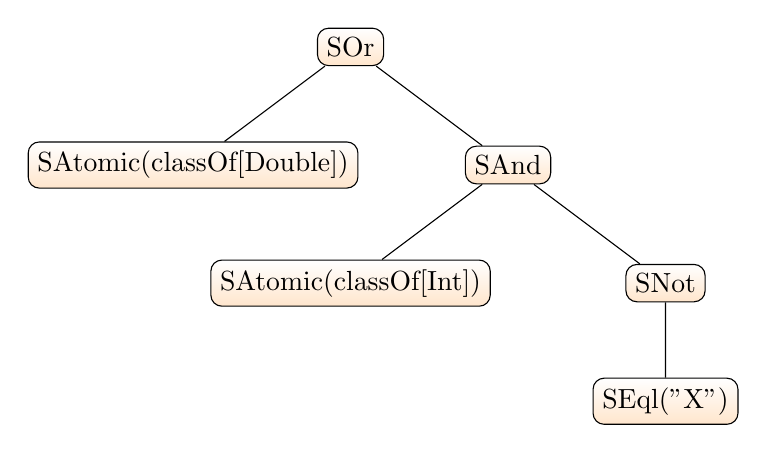
\begin{tikzpicture}[sibling distance=10em,
  every node/.style = {shape=rectangle, rounded corners,
    draw, align=center,
    top color=white, bottom color=orange!20}]]
    \tikzstyle{level 1}=[sibling distance=40mm]
    \tikzstyle{level 2}=[sibling distance=40mm]
    \tikzstyle{level 3}=[sibling distance=40mm]
  \node {SOr}
    child { node {SAtomic(classOf[Double])} }
    child { node {SAnd}
      child { node {SAtomic(classOf[Int])} }
      child { node {SNot} 
        child { node {SEql("X")} } } } ;
\end{tikzpicture}
\end{document}
